% Chapter 1

\chapter{Introducción general} % Main chapter title

\label{Chapter1} % For referencing the chapter elsewhere, use \ref{Chapter1}
\label{IntroGeneral}

%----------------------------------------------------------------------------------------

% Define some commands to keep the formatting separated from the content
\newcommand{\keyword}[1]{\textbf{#1}}
\newcommand{\tabhead}[1]{\textbf{#1}}
\newcommand{\code}[1]{\texttt{#1}}
\newcommand{\file}[1]{\texttt{\bfseries#1}}
\newcommand{\option}[1]{\texttt{\itshape#1}}
\newcommand{\grados}{$^{\circ}$}

%----------------------------------------------------------------------------------------

% Breve descripción del capítulo
En este capítulo se presenta una introducción general al trabajo final, en el cual se describen los antecedentes, la motivación, los objetivos y alcance del trabajo. Además, se presenta el estado del arte en emuladores de sistemas espaciales.

%----------------------------------------------------------------------------------------
\section{Desarrollo de simuladores espaciales y emuladores}
\label{sec:desarrollo_simuladores_emuladores}

% Breve introducción al proceso de desarrollo de simuladores espaciales y uso especifico de emuladores con dicho propósito.
% Se va a incluir imágenes de microprocesadores espaciales.

Para productos de ámbito espacial, como lo son los satélites, muchas veces es difícil, y en ocasiones imposible, generar escenarios realistas para pruebas de los elementos que los componen. Ya sea por no poder generar las mismas condiciones ambientales, o porque la naturaleza de la maniobra que se busca probar implicaría un daño a los equipos bajo revisión.

Otro desafío que se presenta es la escasez de hardware disponible para realizar dichas pruebas, ya que los componentes espaciales no se suelen tener en grandes cantidades, y suelen ser caros. Haciendo que el acceso a dichos recursos sea limitado.

En este contexto, es común replicar los elementos de interés de manera programada, cumpliendo con cierto grado de representatividad. De manera tal que se comporten de la manera más similar posible a su contraparte física. Estos elementos, íntegramente desarrollados en software, se los denominan emulados o simulados. Uno de los componentes que suele generar mayor interés para su simulación es el procesador de la computadora a bordo.

El término computadora a bordo (OBC, por las siglas en inglés de \textit{On Board Computer}) suele referirse a la unidad en la que se ejecuta el software a bordo (OBSW, por sus siglas en inglés de \textit{On Board Software}) y su rol principal es la orquestación del resto de subsistemas en el satélite. Esto incluye recolectar información de los periféricos conectados, analizarla y tomar las decisiones y acciones apropiadas cuando sea requerido.

En la figura \ref{fig:simu_emu} se muestra la relación entre simuladores, emuladores y software de vuelo. Los simuladores satelitales son más abarcativos e incluyen todos los subsistemas simulados del satélite, entre ellos suele encontrarse el emulador de microprocesador. El emulador, por otro lado, se enfocan en reproducir el comportamiento del microprocesador específico a la misión. Por último, el software de vuelo es el software que se ejecuta en la OBC del satélite, y es el software que se busca probar en los emuladores de microprocesadores.

\begin{figure}[htbp]
	\centering
	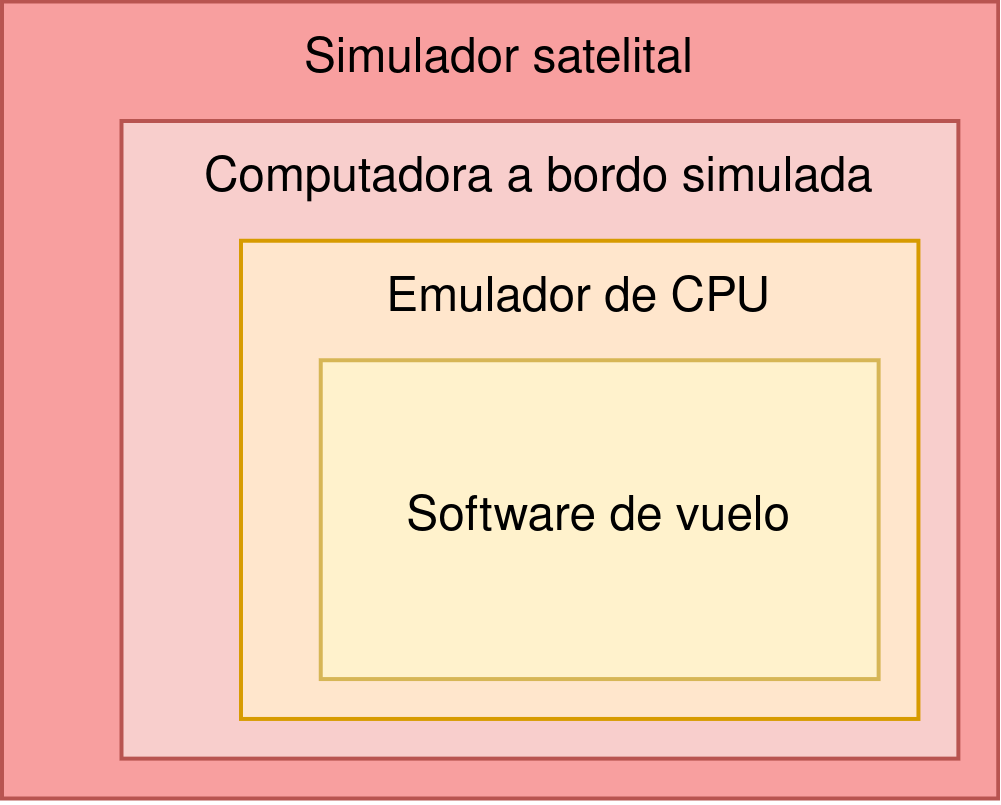
\includegraphics[width=.6\textwidth]{./Figures/simu_emu}
	\caption{Relación entre simuladores, emuladores y software de vuelo.}
	\label{fig:simu_emu}
\end{figure}

\newpage

En el caso de los satélites, la OBC suele estar compuesta por un microprocesador, memoria y periféricos, los últimos suelen variar dependiendo de la misión. El microprocesador es el encargado de ejecutar el OBSW, y es el componente que se busca emular en este trabajo. En la figura \ref{fig:procesadores} se muestran dos microprocesadores de uso espacial, el GR712RC \citep{GR712RC} y el UT700 \citep{UT700}. Ambos utilizan la arquitectura SPARC V8 \citep{SPARC}, que es la arquitectura que se desarrolló en este trabajo.

% TODO: Agregar referencia a Gaisler.

\vspace{1cm}

\begin{figure}[!htpb]
     \centering
     \begin{subfigure}[b]{0.4\textwidth}
         \centering
         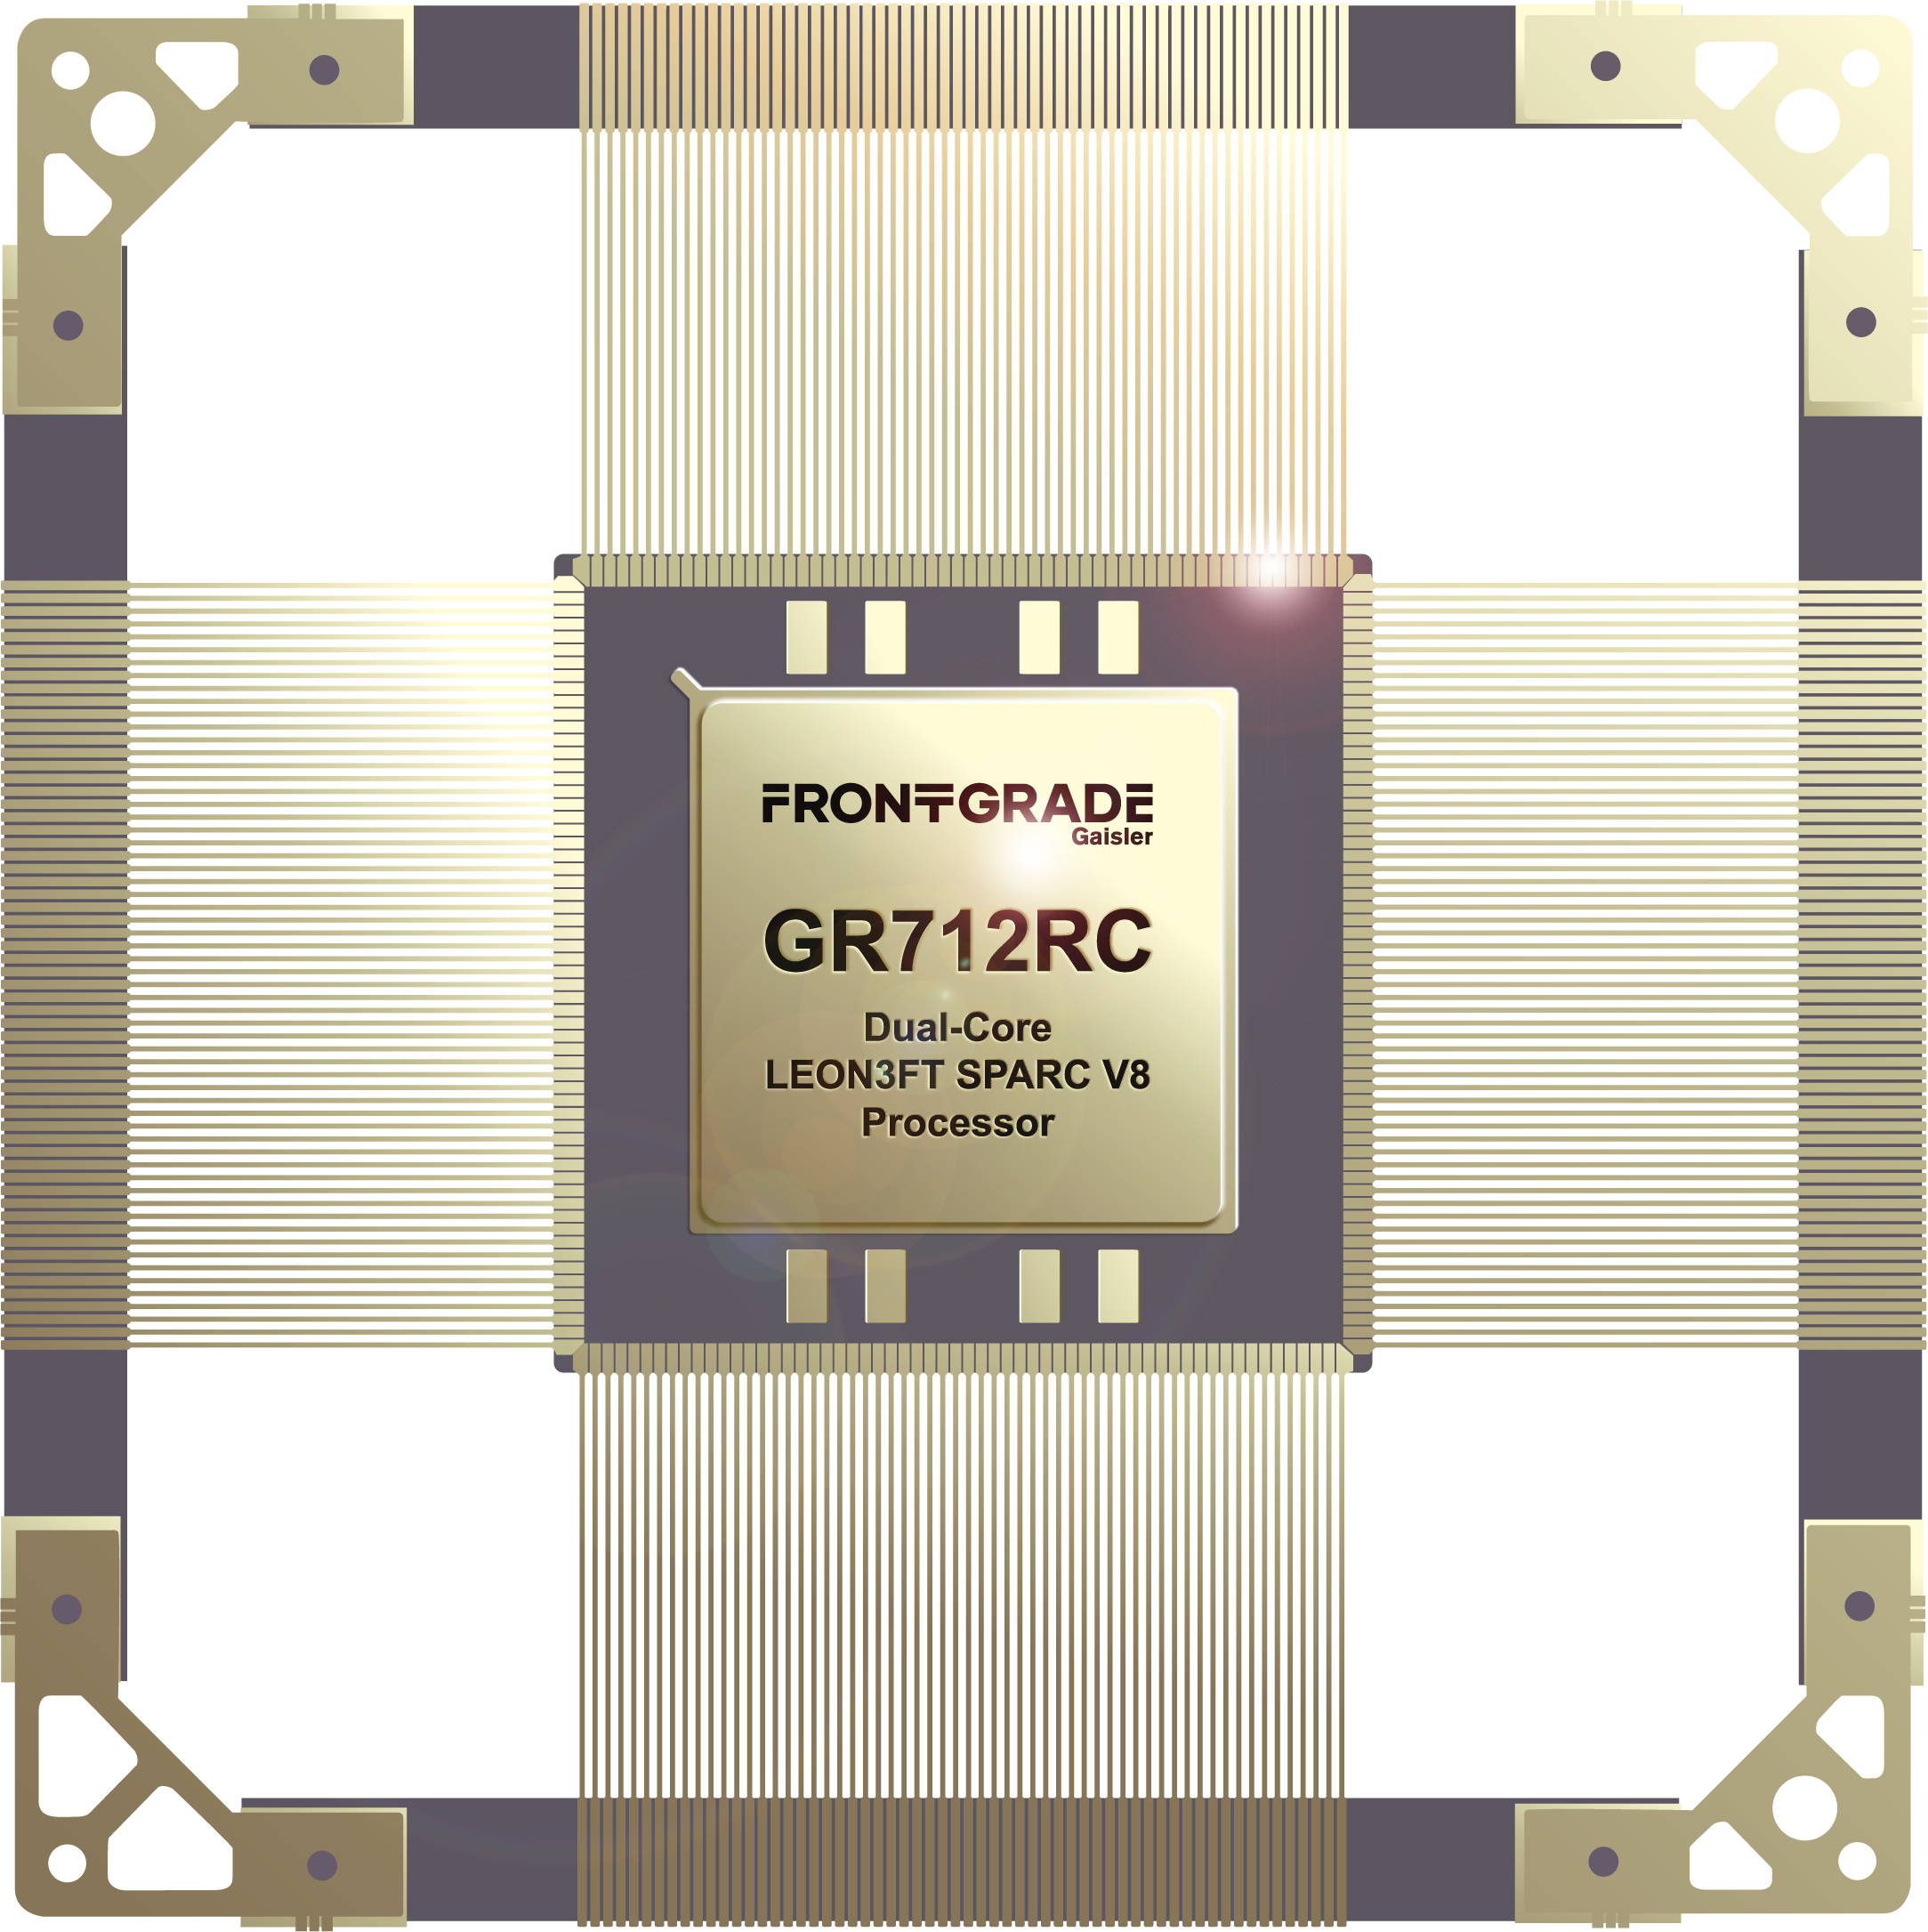
\includegraphics[width=.85\textwidth]{./Figures/gr712rc}
         \caption{Procesador GR712RC.}
         \label{fig:procesadores1de2}
     \end{subfigure}
     \hfill
     \begin{subfigure}[b]{0.50\textwidth}
         \centering
         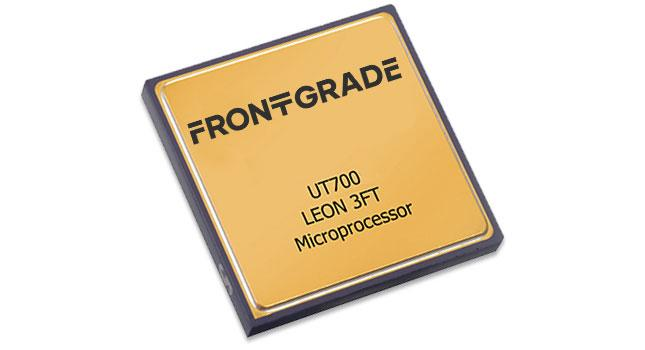
\includegraphics[width=1.28\textwidth]{./Figures/ut700}
         \caption{Procesador UT700.}
         \label{fig:procesadores2de2}
     \end{subfigure}
        \caption{Ejemplo de procesadores de uso espacial.\protect\footnotemark}
        \label{fig:procesadores}
\end{figure}

\footnotetext{Imágenes tomadas de \url{https://www.gaisler.com/}}

\vspace{1cm}

\newpage

Cabe aclarar que el desarrollo de un emulador de microprocesador no es trivial, ya que se debe replicar el comportamiento del microprocesador físico ciclo a ciclo, incluyendo sus instrucciones, registros, y comunicación con los periféricos. Además, se debe tener en cuenta que el microprocesador real puede tener características específicas que no se encuentran en otros microprocesadores, lo que puede dificultar la tarea de emulación.

Dado que el presente desarrollo se realiza en el marco de un posgrado, no se buscó replicar todas las funcionalidades del microprocesador, sino que un subconjunto de las mismas. En particular, el desarrollo se enfocó en la emulación de las instrucciones básicas del microprocesador GR712RC, omitiendo múltiples instrucciones y periféricos.

\section{Estado del arte}
\label{sec:estado_arte}

En la actualidad, existen dos grandes grupos de emuladores de microprocesadores: los emuladores de microprocesadores de propósito general y los de propósito específico.

Los emuladores de propósito general son aquellos que buscan emular una amplia variedad de microprocesadores de manera genérica, es decir, sin tener en cuenta las características específicas de cada microprocesador. Estos emuladores suelen ser muy complejos y suelen tener un rendimiento inferior a los emuladores de propósito específico, ya que su implementación debe ser lo más abarcativa posible. En particular, los emuladores de propósito general suelen ser utilizados en el desarrollo donde el rendimiento no es un factor crítico.

Un ejemplo de este tipo de emuladores es QEMU \citep{QEMU}, un emulador de código abierto que permite emular múltiples arquitecturas de microprocesadores, incluyendo x86, ARM, SPARC y otros. QEMU es un emulador muy popular y es utilizado en múltiples proyectos de software libre y de código abierto. Teniendo una comunidad activa de desarrolladores y usuarios. Haciendo que sea una opción muy atractiva para su uso.

Por otro lado, los emuladores de propósito específico son aquellos que buscan emular un microprocesador específico. Estos emuladores suelen ser más simples que los emuladores de propósito general, ya que no buscan generalidad, sino que buscan emular un microprocesador específico de la manera más precisa y eficiente posible. Pudiendo utilizar optimizaciones específicas que podrían romper con la compatibilidad con otros microprocesadores.

Una clara ventaja de este tipo de emuladores, además de su rendimiento, es que suelen ser más fáciles de utilizar y de integrar con otros sistemas, porque están diseñados desde un inicio para ser embebidos en otros sistemas. Lo que es de suma importancia en el desarrollo de sistemas espaciales, ya que gran parte del desarrollo suele hacerse dentro de la misma organización.

A continuación, en la tabla \ref{tab:comparacion_emuladores} se muestra una tabla comparativa entre emuladores de propósito general y de propósito específico.

\begin{table}[h]
	\centering
	\caption[Tipos de emuladores]{Comparación entre emuladores de propósito general y de propósito específico.}
	\begin{tabular}{l c c}
		\toprule
		\textbf{Emuladores específicos} & \textbf{Emuladores genéricos} \\
		\midrule
		Usualmente privativos y pagos & Solidas opciones gratis disponibles	\\
		Alto rendimiento	 & No enfocado en el rendimiento  \\
		Alta integrabilidad	 & Baja integrabilidad	 \\
		Soporte limitado & Comunidades activas y código abierto	 \\
		\bottomrule
		\hline
	\end{tabular}
	\label{tab:comparacion_emuladores}
\end{table}



\section{Objetivos y alcance}
\label{sec:objetivos_alcance}

En esta sección se presentan los objetivos y alcance del trabajo final. Además, se presenta el alcance del trabajo, en el cual se describen las limitaciones y restricciones del trabajo.


\subsection{Objetivos}
\label{subsec:objetivos}

El objetivo de este trabajo es el diseño e implementación de un emulador de microprocesador LEON3 desarrollado para la empresa INVAP. SE, pensado para su uso en simulaciones espaciales. El emulador debe ser capaz de emular todas las instrucciones necesarias de un bootloader, e instrucciones de propósito general tal como operaciones de adición, sustracción, y acceso a memoria. Además, el trabajo de contar con un modelo de memoria RAM, y operaciones de carga de binarios en dicha memoria.

Las operaciones de lectura y escritura deberán acceder a una memoria RAM emulada, y deberán ser accesibles a través de la API expuesta para la interacción con el emulador.

Otro objetivo del presente trabajo es la creación de manual de usuario de la herramienta, que permita a futuros desarrolladores entender el uso de la herramienta y su integración con otros sistemas.

\subsection{Alcance}
\label{subsec:alcance}

El alcance del trabajo se limita a la emulación de un subconjunto de instrucciones del microprocesador LEON3, omitiendo múltiples instrucciones y periféricos. El trabajo no busca ser una herramienta finalizada, sino que busca ser una base sólida para futuros desarrollos. Dadas estas condiciones, el alcance del trabajo se limita a los siguientes puntos:

\begin{itemize}
  %% \item Desarrollo del software de emulación.
\item El objetivo principal es el desarrollo del software de emulación. Las instrucciones seleccionadas para ser implementadas son:
  \begin{enumerate}

    \item \texttt{UNIMP}: Genera un interrupción de procesador.
    \item \texttt{Bicc}: Salto condicional (Números enteros).
    \item \texttt{SETHi}: Escritura de los 22bits mas significativos de un registro.
    \item \texttt{FBfcc}: Salto condicional (Números punto flotante).
    \item \texttt{CBfcc}: Salto condicional (Códigos de condición).

    \item \texttt{CALL}: Llamada a subrutina.

    \item \texttt{ADD}: Adición.
    \item \texttt{ADDcc}: Adición con código de condición.
    \item \texttt{ADDX}: Adición con retorno de carro.

    \item \texttt{SUB}: Sustracción.
    \item \texttt{SUBcc}: Sustracción con código de condición.
    \item \texttt{SUBX}: Sustracción con retorno de carro.

    \item \texttt{AND}: Operación \texttt{AND} lógica.
    \item \texttt{ANDcc}: Operación \texttt{AND} lógica con actualización de código de condición.
    \item \texttt{ANDN}: Operación de \texttt{AND} negada lógica.

    \item \texttt{OR}: Operación \texttt{OR} lógica.
    \item \texttt{XOR}: Operación de \textit{exclusive or}.
    \item \texttt{ORcc}: Operación \texttt{OR} lógica con actualización de código de condición.

    \item \texttt{SLL}: Desplazamiento lógico a la izquierda.
    \item \texttt{SRL}: Desplazamiento lógico a la derecha.
    \item \texttt{SRA}: Desplazamiento aritmético a la derecha.

    \item \texttt{RDPSR}: Lectura del registro de estado del procesador.

    \item \texttt{RDY\_RDASR}: Lectura del registro \texttt{Y} del procesador.

    \item \texttt{WRY}: Escritura del registro \texttt{Y} del procesador.
    \item \texttt{WRPSR}: Escritura del registro \texttt{PSR} del procesador.
    \item \texttt{WRWIM}: Escritura del registro \texttt{WIM} del procesador.
    \item \texttt{WRTBR}: Escritura del registro \texttt{TBR} del procesador.

    \item \texttt{TICC}: Interrupción en código de condición de enteros.

    \item \texttt{JMPL}: Salto incondicional.
    \item \texttt{FLUSH}: Limpieza de operaciones pendientes.
    \item \texttt{SAVE}: Guardado de ventana de procesamiento.
    \item \texttt{RESTORE}: Carga de ventana de procesamiento.

  \end{enumerate}

  Para más detalle sobre cada instrucción se recomienda leer el manual de arquitectura SPARC V8 \citep{SPARC}.

  \item Desarrollo de operaciones esperables de un emulador de microprocesador. Tales como la carga de binarios en RAM para su ejecución, la ejecución de instrucciones, y la interacción con periféricos.
  \item Creación de API para la interacción con el emulador. Este es el único punto de interacción que tendrá con el usuario con la aplicación, por lo que es de especial importancia su correcta documentación.
  \item Desarrollo de modelo de memoria RAM, capaz de interactuar tanto con la API expuesta el usuario para lecturas y escrituras arbitrarias, como para el modelo de procesador desarrollado.
  \item Desarrollo de mecanismo de depuración de la herramienta. Tal como el volcado del estado del procesador a archivos de formato CSV, mostrando el estado paso a paso durante una ejecución.
  \item Manual de usuario de la herramienta. Este manual deberá ilustrar en detalle el uso esperado de la herramienta, también deberá exponer sus limitaciones.
\end{itemize}
